\documentclass[main.tex]{subfiles} % Subfile-Class

%==============================================================================%
%                                   Subfile                                    %
%==============================================================================%

\begin{document}

% Template

\subsubsection{Greifeinheit}

\subsubsection*{Anforderungen}

Die Greifkraft ist so auszulegen, dass das Hindernis zuverlässig und sicher gegriffen werden kann.
Insbesondere sind die Haftreibung zwischen Greiffläche und Objekt sowie die Anpresskraft zu berücksichtigen,
um ein Abrutschen während des Transports zu verhindern. Die Höhenverstellung des Greifers ist auf das Gesamtgewicht
der zu bewegenden Last abzustimmen. Dazu zählen das Gewicht des Hindernisses, des Greifers selbst sowie der
mitgeführten Elektronik. Eine Wiederholgenauigkeit ist für den gesamten Bewegungsablauf des Greifers erforderlich.
Diese stellt sicher, dass das Hindernis stets innerhalb des geforderten Toleranzbereichs platziert wird und die
Funktionalität des Gesamtsystems nicht beeinträchtigt wird. Das Gewicht der Greifereinheit ist möglichst gering 
zu halten, um das Gesamtgewicht des Fahrzeugs zu minimieren. Eine reduzierte Masse ist insbesondere bei den bewegten
Teilen des Greifers von Bedeutung, da sie direkten Einfluss auf die Auswahl der Antriebskomponenten, die erreichbare
Geschwindigkeit sowie die Energieeffizienz des Systems hat.


\subsubsection*{Konstruktive Umsetzung}

Die Abbildung~\ref{fig:Greifereinheit} zeigt das realisierte Greiferkonzept des Roboters.
Es wurde auf Basis der Erkenntnisse aus PREN1 weiterentwickelt und in PREN2 gezielt optimiert.
Das Greiferkonzept wurde überwiegend aus PLA im 3D-Druckverfahren gefertigt.
Dies ermöglichte eine schnelle und flexible Umsetzung sowie einfache Anpassungen über Anpassungen
über mehrere Iterationen hinweg. Die nachfolgende Beschreibung erläutert die Funktionsweise des Greifers im Detail.

\begin{figure}[H]
    \centering
    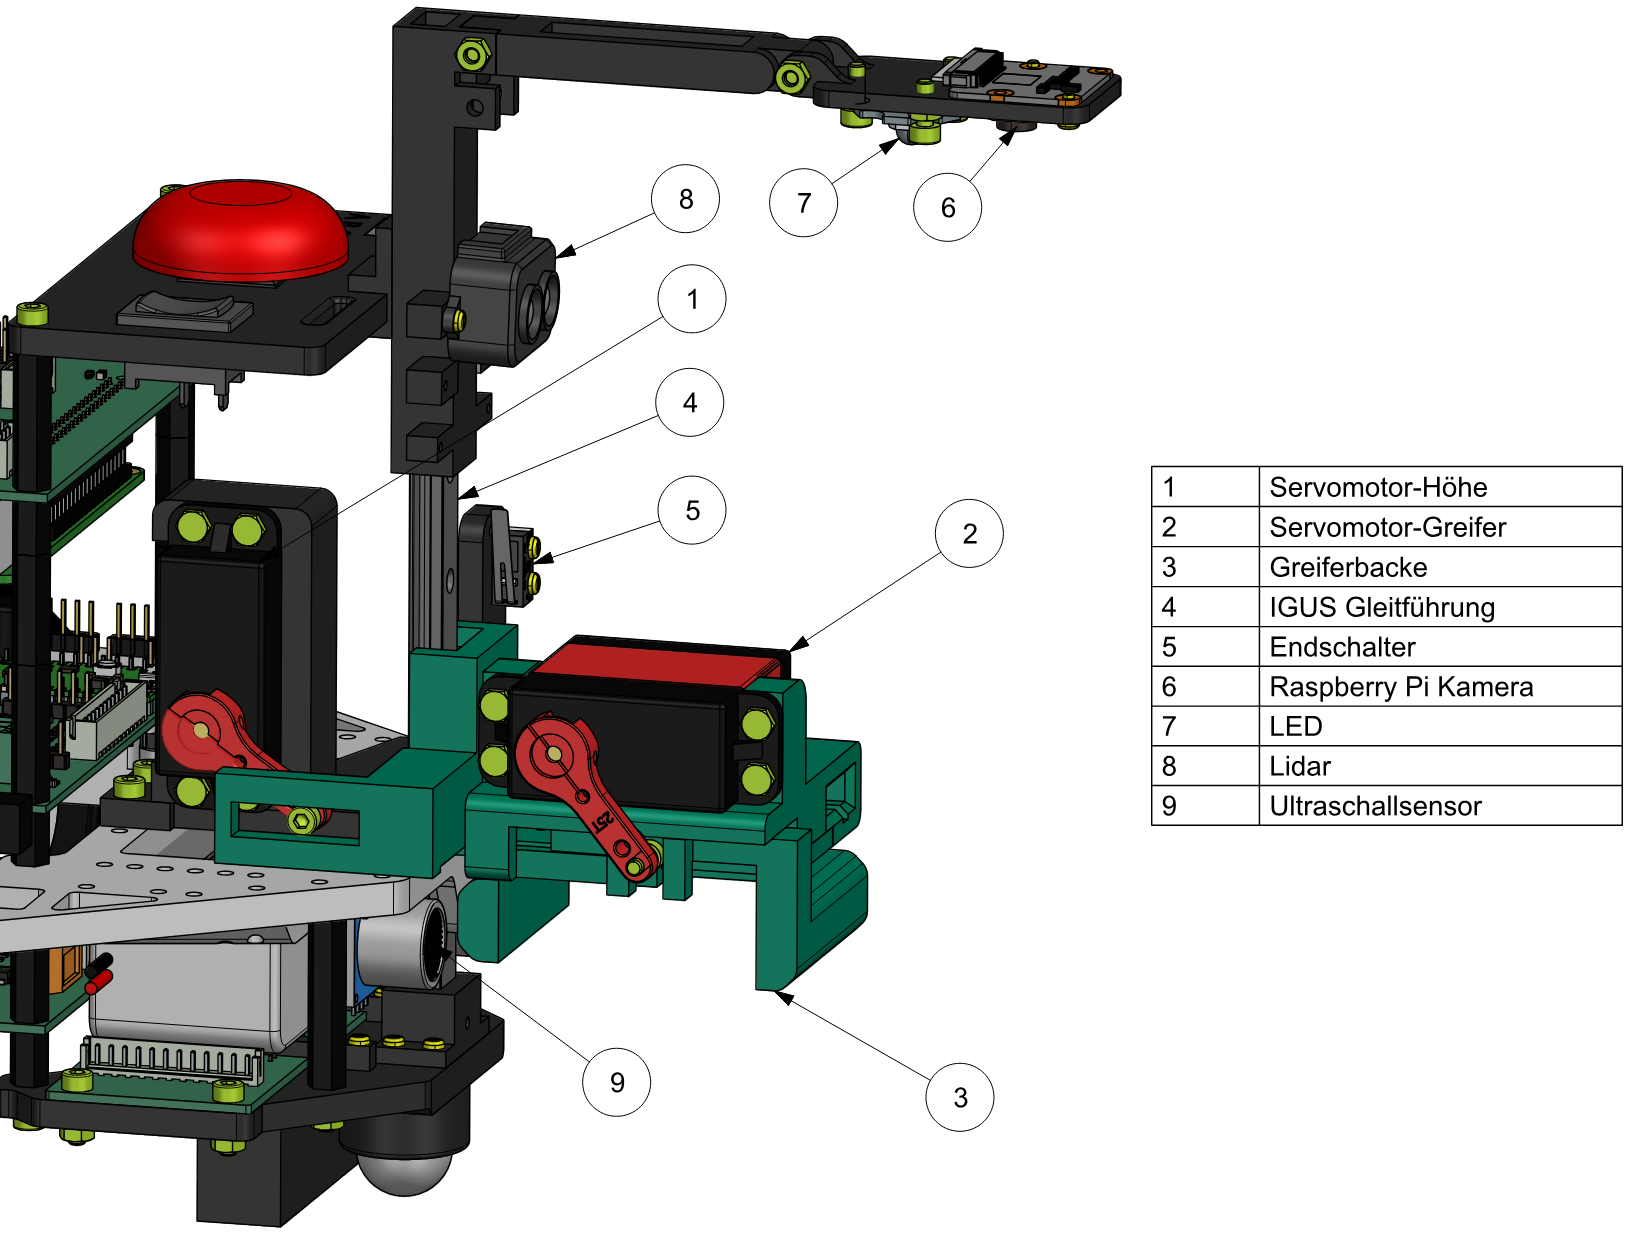
\includegraphics[width = 0.9\linewidth]{./fig_Mechanik/Greifereinheit_PREN2.png}
    \caption{Greifereinheit dargestellt in Siemens NX}~\label{fig:Greifereinheit}
\end{figure}

%==============================================================================%

\newpage

Der Greifer besitzt zwei gegenüberliegende Backen, die sich parallel zueinander bewegen,
um das Hindernis sicher zu greifen. Die Bewegung wird durch einen Servomotor gesteuert.
Ein Hebel, angetrieben vom Servomotor, verschiebt eine der beiden Backen horizontal.
Diese Backe ist mit einer Zahnstange versehen, die ein innenliegendes Zahnrad (Abbildung ~\ref{fig:Zahnrad}) antreibt.
Das Zahnrad überträgt die Bewegung auf die gegenüberliegende Backe, wodurch sich beide
synchron, jedoch in entgegengesetzten Richtungen bewegen.

\begin{figure}[H]
    \centering
    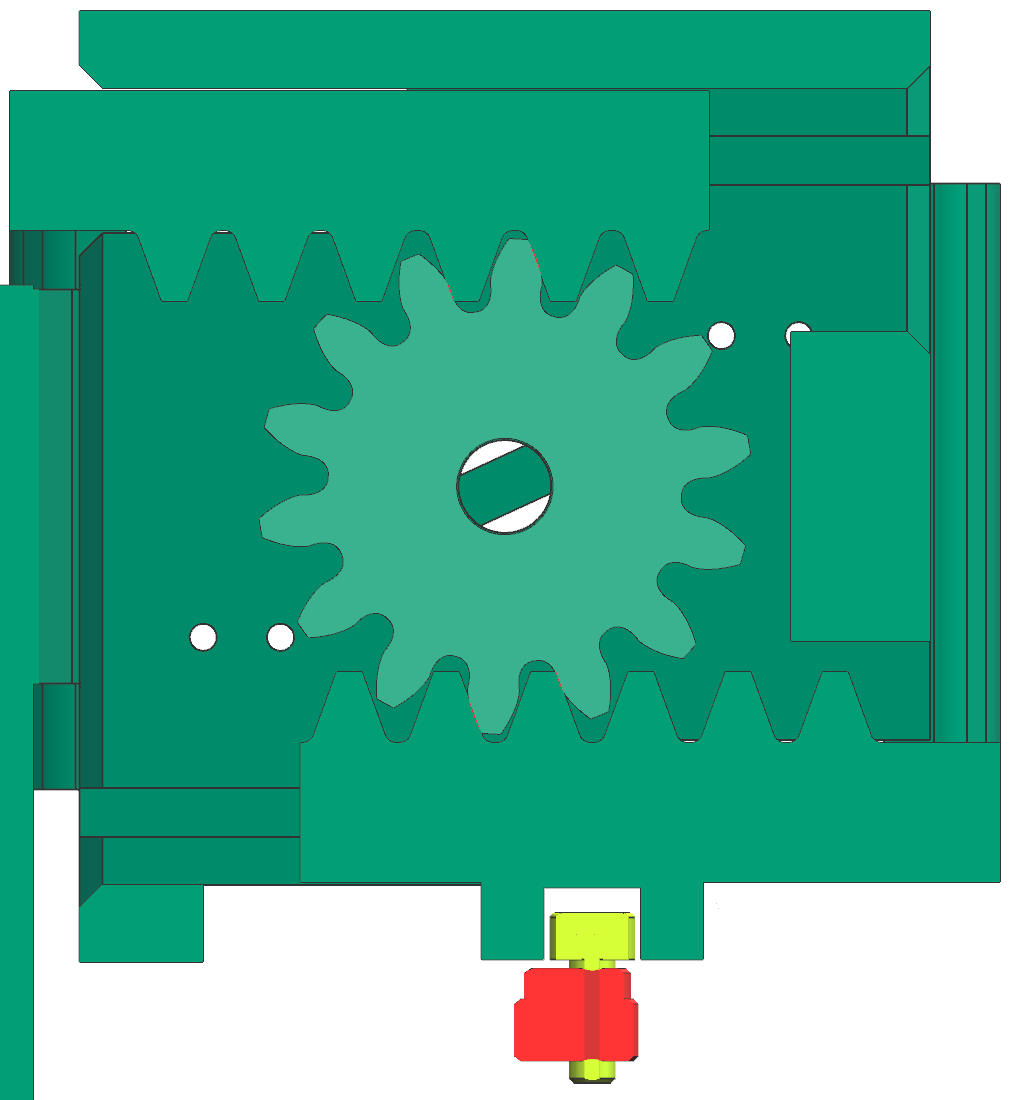
\includegraphics[width = 0.45\linewidth]{./fig_Mechanik/Zahnrad.png}
    \caption{innenliegendes Zahnrad dargestellt in Siemens NX}~\label{fig:Zahnrad}
\end{figure}

\begin{figure}[H]
    \centering
    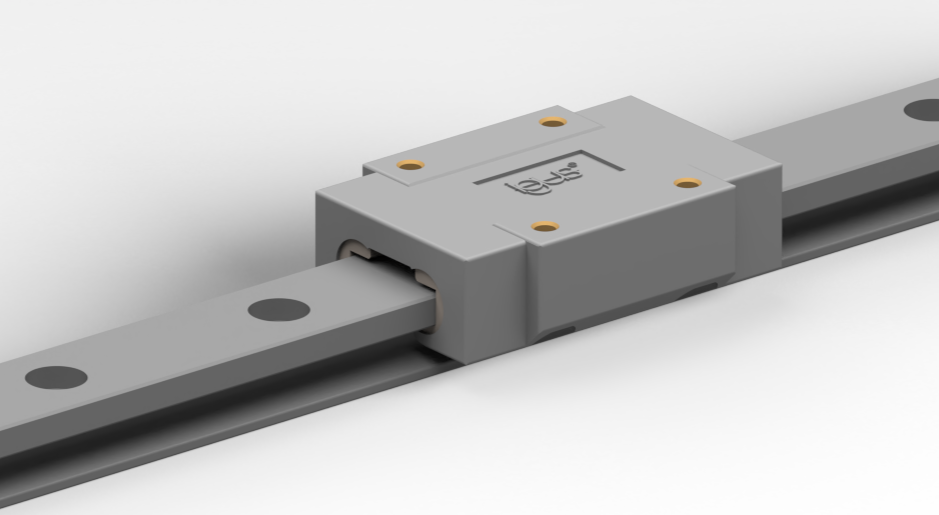
\includegraphics[width = 0.65\linewidth]{./fig_Mechanik/IGUS.png}
    \caption{IGUS Gleitführung dargestellt in Siemens NX}~\label{fig:IGUS}
\end{figure}

Auch die Höhenverstellung erfolgt
über einen Servomotor, der den gesamten Greifer entlang einer Gleitführung von IGUS (Abbildung ~\ref{fig:IGUS}) vertikal bewegt.
Das für das Greifen erforderliche Drehmoment beträgt 0.235 $ \text{Nm}$,
für die Höhenverstellung 0.2 $\text{Nm}$. Diese Werte wurden mit den folgenden Formeln berechnet:

\[
    M_{Greifer} = \frac{m \cdot g}{\mu_{\text{hr}}} \cdot Hebel \cdot Sicherheit
\]

\[
    M_{Hoehe} = (m_{Hindernis} + m_{Elektronik} + m_{Greifer}) \cdot Hebel \cdot Sicherheit
\]

%==============================================================================%

\newpage

Zur Begrenzung der Endpositionen der Höhenverstellung sind zwei Endschalter verbaut.  
Diese dienen sowohl der Positionsrückmeldung als auch dem Schutz vor einem Überdrehen des Servomotors.  
Damit wird sichergestellt, dass der Greifer stets die korrekte Höhe erreicht und mechanische Beschädigungen vermieden werden.

\subsubsection*{Greiferablauf}

Die Abbildung~\ref{fig:Greiferablauf} zeigt den Ablauf des Greifvorgangs in mehreren Bildern.
Die Bewegung des Motors werden mit einem gelben Pfeil dargestellt:

\begin{figure}[H]
    \centering
    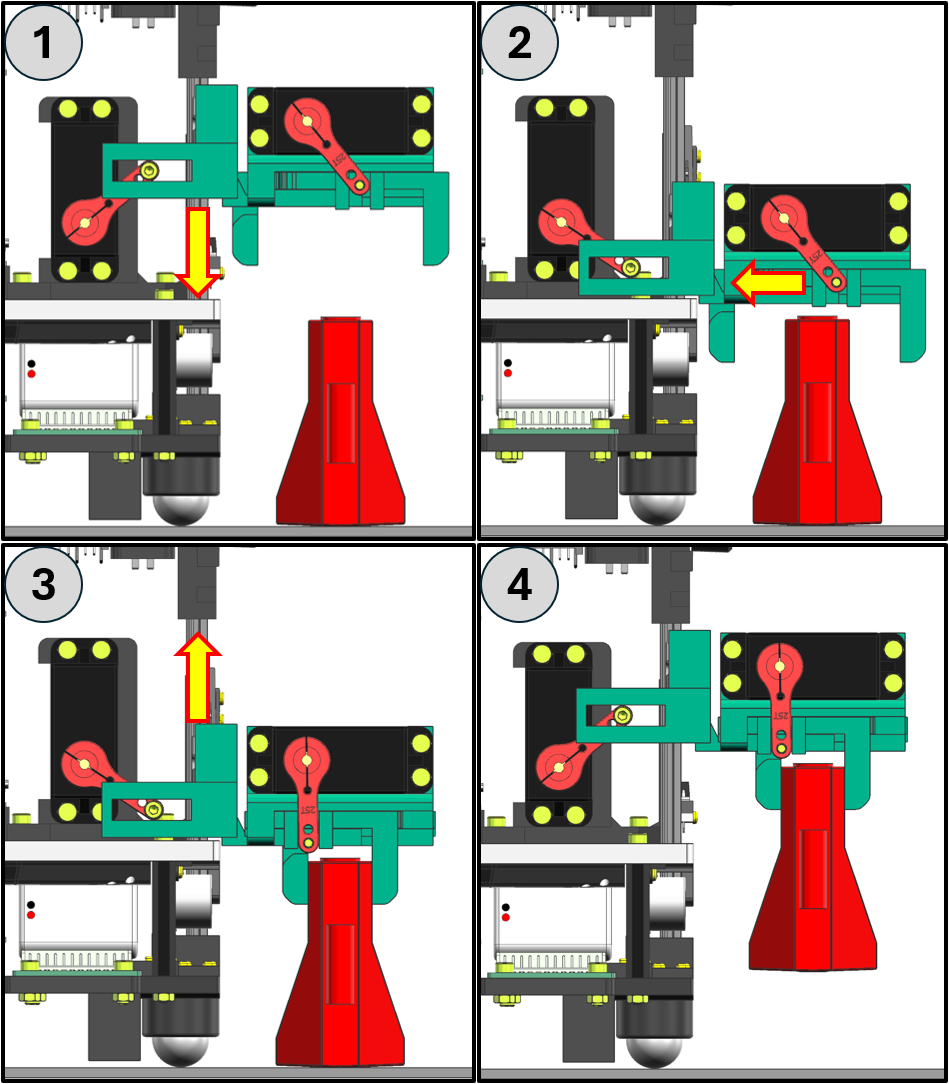
\includegraphics[width = 0.85\linewidth]{./fig_Mechanik/Greiferablauf_PREN2.png}
    \caption{Greiferablauf dargestellt in Siemens NX}~\label{fig:Greiferablauf}
\end{figure}


\begin{description}
    \item[Positionierung der Greifeinheit] Nach der Erkennung eines Hindernisses durch den 
        Ultraschallsensor bewegt der linke Servomotor 
        die Greifeinheit entlang einer Gleitführung von Position 1 zu Position 2 nach unten, 
        bis der untere Endschalter erreicht ist.

    \item[Greifen des Hindernisses] Anschliessend bewegt der rechte Servomotor die Greifbacken 
        horizontal von Position 2 zu Position 3, 
        sodass sich beide Backen parallel schliessen und das Hindernis sicher erfassen.

    \item[Anheben des Hindernisses] Im letzten Schritt dreht der linke Servomotor die 
        Greifeinheit von Position 3 zu Position 4 nach oben, 
        bis der obere Endschalter erreicht ist.  
        Dadurch wird das Hindernis vom Boden angehoben und ein sicherer Transport ermöglicht.

\end{description}



\subsubsection{Sensorikplatzierung}

In diesem Abschnitt wird die Positionierung der Sensoren erläutert.

\begin{description}
    \item[Raspberry Pi Kamera – Knotenpunkt] Die Raspberry-Pi-Kamera ist in einer Höhe von \textbf{200 mm} montiert. In dieser Position kann 
        sie sowohl die \textbf{80–120 mm} grossen Knotenpunkte als auch die Abgänge zuverlässig erfassen. 
        Zur Sicherstellung konstanter Lichtverhältnisse ist zusätzlich eine LED verbaut.
    
    \item[LiDAR – Pylonerkennung] Der LiDAR-Sensor ist in einer Höhe von \textbf{165 mm} und in einem Winkel von \textbf{2°} montiert. 
        Diese Anordnung ermöglicht die Detektion von Pylonen in einer Entfernung von bis zu \textbf{2 Metern}. 
        Die gewählte Montagehöhe stellt sicher, dass innerhalb dieses Erfassungsbereichs keine unerwünschten 
        Streueffekte auftreten, die zu Fehlmessungen führen könnten. Eine detaillierte Beschreibung der 
        Funktionsweise findet sich in Kapitel~\ref{sec:Sensorik_Lidar}.
    
    \item[Ultraschallsensor – Hinderniserkennung] Der Ultraschallsensor ist in einer Höhe von \textbf{50 mm} angebracht und dient der frühzeitigen 
        Erkennung von Hindernissen, um Kollisionen mit dem Roboter zu vermeiden. Zudem stellt er sicher, 
        dass der Roboter exakt an der vorgesehenen Position stoppt, um das Hindernis anzuheben. Die genaue 
        Funktionsweise wird in Kapitel~\ref{sec:Sensorik_Ultraschall} ausführlich beschrieben.

\end{description}


\end{document}
